\clearpage


\chapter{Исследовательская часть}\label{ch:-}
В этом разделе приведен сравнительный анализ алгоритмов по времени выполнения.


\section{Технические характеристики ЭВМ}\label{sec:--2}
Все замеры проводились на ЭВМ при использовании микроконтроллера $STM32{[3]}$. Характеристики ЭВМ приведены ниже:
\begin{itemize}
    \item процессор: AMD Ryzen™ 7--5800H with Radeon™ Graphics × 16;
    \item ОС: 64-разрядная операционная система Ubuntu 24.04.1 LTS;
    \item оперативная память: 16,0 ГБ.
\end{itemize}


\section{Сравнение алгоритмов}
В таблице~\ref{tbl:mult_time} приведено время работы алгоритмов в секундах.
Для повышения точности результатов проводилось 200 замеров.

\begin{table}[h]
	\begin{center}
	\caption{\label{tbl:mult_time} Сравнение алгоритмов умножения матриц по времени выполнения}
	\begin{tabular}{|c|r|r|r|}
		\hline
		Размер квадратной матрицы & Стандартный & Виноград & Оптимизированный
		\\ \hline
		10 & 0.00015 & 0.00017 & 0.00020
		\\ \hline
		30 & 0.0020 & 0.0016 & 0.0020
		\\ \hline
		50 & 0.009 & 0.009 & 0.009
		\\ \hline
		70 & 0.017 & 0.016 & 0.016
		\\ \hline
		90 & 0.035 & 0.032 & 0.030
		\\ \hline
		110 & 0.041 & 0.037 & 0.036
		\\ \hline
	\end{tabular}
	\end{center}
\end{table}

\clearpage
На графике~\ref{grph:mult_time} приведена визуализация результатов.
\begin{figure}[H]
    \centering
    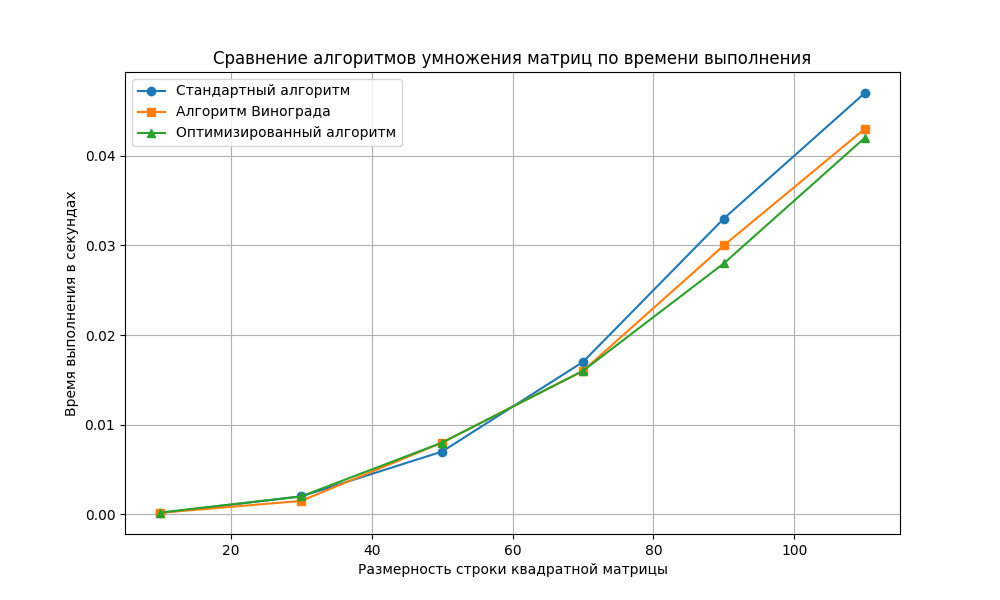
\includegraphics[width=1\linewidth]{images/performance_plot}
    \caption{Сравнения для каждого элемента в алгоритме полного перебора}
    \label{grph:mult_time}
\end{figure}

\section*{Вывод}

Хотя оптимизированный алгоритм Винограда имеет большую теоретическую сложность по сравнению со стандартным,
он работает быстрее при умножении матриц размерностью от 40 элементов (примерно на 10\%).
Оптимизированный алгоритм работает быстрее неоптимизированной версии на размерностях матриц больше 70.

\clearpage